\section{Class diagram}
\subsection{Class diagram của hệ thống}
\begin{figure}[H]
    \centering
    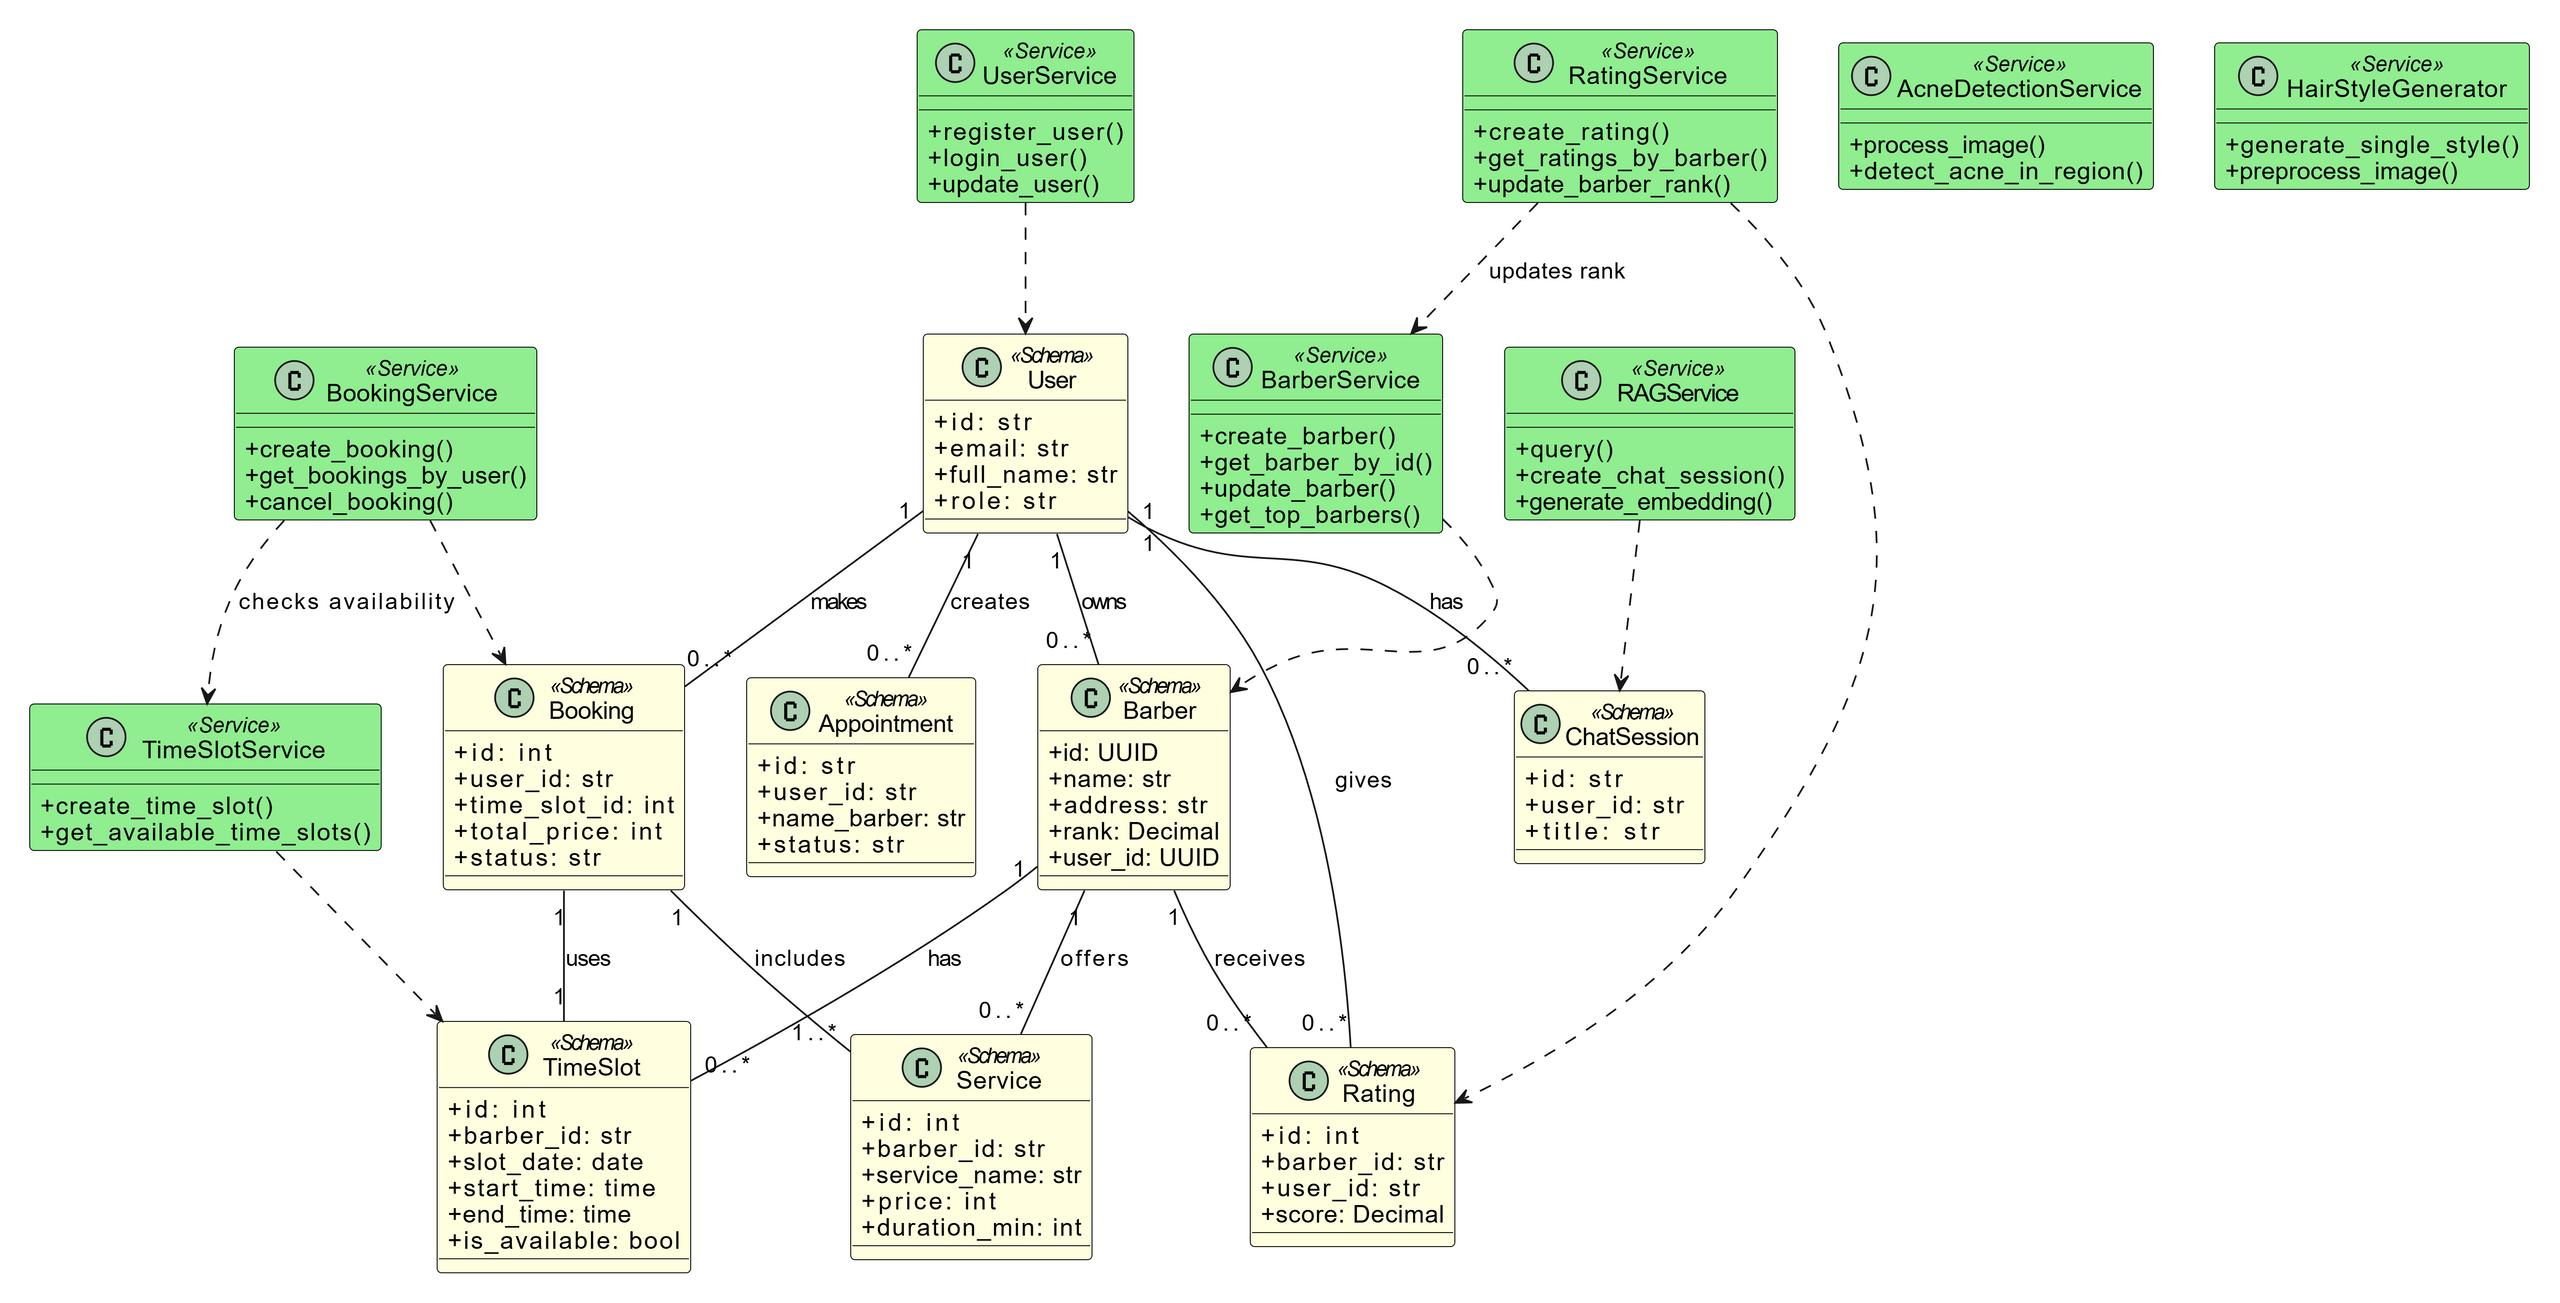
\includegraphics[width=1\textwidth]{figures/class.jpg}
    \caption{Class diagram của hệ thống}
    \label{fig:class}
\end{figure}

Class Diagram mô tả cấu trúc tĩnh của hệ thống BarberGo, bao gồm các lớp Schema (đại diện cho entities/models) và các lớp Service (đại diện cho business logic layer). Thiết kế tuân theo kiến trúc Three-Tier với tách biệt rõ ràng giữa data models và business logic.

\subsection{Nhóm lớp Schema (Data Models)}

Các lớp Schema đại diện cho các thực thể trong cơ sở dữ liệu, được thiết kế dựa trên Pydantic models để đảm bảo type safety và data validation.

\subsubsection{Core Schemas}

\textbf{User:} Đại diện cho người dùng hệ thống với các thuộc tính \texttt{id} (str), \texttt{email} (str), \texttt{full\_name} (str), \texttt{role} (str: customer/barber/admin). Có quan hệ 1-N với Barber, Booking, Rating, Appointment và ChatSession.

\textbf{Barber:} Thông tin barber shop với \texttt{id} (UUID), \texttt{name} (str), \texttt{address} (str), \texttt{rank} (Decimal), \texttt{user\_id} (UUID). Quan hệ N-1 với User, 1-N với Service, TimeSlot và Rating.

\textbf{Service:} Dịch vụ cung cấp với \texttt{id} (int), \texttt{barber\_id} (str), \texttt{service\_name} (str), \texttt{price} (int), \texttt{duration\_min} (int). Quan hệ N-1 với Barber và M-N với Booking.

\textbf{TimeSlot:} Khung giờ làm việc với \texttt{id} (int), \texttt{barber\_id} (str), \texttt{slot\_date} (date), \texttt{start\_time} (time), \texttt{end\_time} (time), \texttt{is\_available} (bool). Quan hệ N-1 với Barber và 1-1 với Booking.

\textbf{Booking:} Lịch hẹn với \texttt{id} (int), \texttt{user\_id} (str), \texttt{time\_slot\_id} (int), \texttt{total\_price} (int), \texttt{status} (str: pending/confirmed/rejected/completed). Quan hệ N-1 với User, 1-1 với TimeSlot, M-N với Service.

\textbf{Rating:} Đánh giá với \texttt{id} (int), \texttt{barber\_id} (str), \texttt{user\_id} (str), \texttt{score} (Decimal: 1-5). Quan hệ N-1 với cả User và Barber.

\textbf{Appointment:} Yêu cầu hợp tác với \texttt{id} (str), \texttt{user\_id} (str), \texttt{name\_barber} (str), \texttt{status} (str: pending/approved/rejected). Quan hệ N-1 với User.

\textbf{ChatSession:} Phiên chat với \texttt{id} (str), \texttt{user\_id} (str), \texttt{title} (str). Quan hệ N-1 với User.

\subsection{Nhóm lớp Service (Business Logic)}

Các lớp Service chứa business logic và orchestrate operations trên data models, implement các use cases của hệ thống.

\subsubsection{Core Services}

\textbf{UserService:} Quản lý user lifecycle với các methods:
\begin{itemize}
    \item \texttt{register\_user()}: Đăng ký tài khoản mới, validate email uniqueness
    \item \texttt{login\_user()}: Xác thực người dùng, tạo session
    \item \texttt{update\_user()}: Cập nhật thông tin profile (avatar, phone, password)
\end{itemize}

\textbf{BarberService:} Quản lý barber shops với các methods:
\begin{itemize}
    \item \texttt{create\_barber()}: Tạo barber shop mới, validate owner
    \item \texttt{get\_barber\_by\_id()}: Lấy thông tin chi tiết barber
    \item \texttt{update\_barber()}: Cập nhật thông tin, services, working hours
    \item \texttt{get\_top\_barbers()}: Lấy danh sách barbers theo rank và location
\end{itemize}

\textbf{TimeSlotService:} Quản lý khung giờ với các methods:
\begin{itemize}
    \item \texttt{create\_time\_slot()}: Tạo khung giờ mới cho barber
    \item \texttt{get\_available\_time\_slots()}: Lấy danh sách khung giờ trống theo ngày và barber
\end{itemize}

\textbf{BookingService:} Xử lý đặt lịch với các methods:
\begin{itemize}
    \item \texttt{create\_booking()}: Tạo booking mới, lock time slot, tính total price
    \item \texttt{get\_bookings\_by\_user()}: Lấy lịch sử bookings của user
    \item \texttt{cancel\_booking()}: Hủy booking, release time slot
\end{itemize}
Dependency: TimeSlotService (kiểm tra availability trước khi book)

\textbf{RatingService:} Quản lý đánh giá với các methods:
\begin{itemize}
    \item \texttt{create\_rating()}: Tạo rating mới, validate booking completed
    \item \texttt{get\_ratings\_by\_barber()}: Lấy danh sách ratings của barber
    \item \texttt{update\_barber\_rank()}: Tính lại rank trung bình, trigger sau mỗi rating
\end{itemize}
Dependency: BarberService (cập nhật rank)

\subsubsection{AI Services}

\textbf{RAGService:} Xử lý chatbot RAG với các methods:
\begin{itemize}
    \item \texttt{query()}: Xử lý query từ user, semantic search documents, generate response
    \item \texttt{create\_chat\_session()}: Tạo session mới cho user
    \item \texttt{generate\_embedding()}: Convert text thành vector embedding (768-dim)
\end{itemize}
Technologies: Google text-embedding-004, Gemini 2.0 Flash, pgvector cosine similarity

\textbf{AcneDetectionService:} Phát hiện mụn với các methods:
\begin{itemize}
    \item \texttt{process\_image()}: Pipeline chính - preprocess, detect, analyze
    \item \texttt{detect\_acne\_in\_region()}: Detect mụn trong vùng face sử dụng YOLOv8 + CNN
\end{itemize}
Technologies: MediaPipe Face Mesh, YOLOv8, MobileNetV2 CNN

\textbf{HairStyleGenerator:} Tạo kiểu tóc với các methods:
\begin{itemize}
    \item \texttt{generate\_single\_style()}: Generate hairstyle sử dụng Stable Diffusion
    \item \texttt{preprocess\_image()}: Face detection, segmentation, mask preparation
\end{itemize}
Technologies: Stable Diffusion 1.5 Inpainting, MediaPipe Face Mesh

\subsection{Quan hệ giữa các lớp}

\subsubsection{Schema Associations}

Các mối quan hệ chính giữa các Schema classes:
\begin{itemize}
    \item User owns (1-N) Barber: Một user có thể sở hữu nhiều barber shops
    \item User makes (1-N) Booking: Một user có thể đặt nhiều lịch hẹn
    \item User gives (1-N) Rating: Một user có thể đánh giá nhiều barbers
    \item Barber offers (1-N) Service: Một barber cung cấp nhiều dịch vụ
    \item Barber has (1-N) TimeSlot: Một barber có nhiều khung giờ
    \item Booking uses (1-1) TimeSlot: Một booking chiếm một khung giờ duy nhất
    \item Booking includes (M-N) Service: Một booking có thể bao gồm nhiều dịch vụ
\end{itemize}

\subsubsection{Service Dependencies}

Các lớp Service có dependency relationships để implement business workflows:
\begin{itemize}
    \item UserService → User: CRUD operations trên User model
    \item BarberService → Barber: CRUD operations trên Barber model
    \item BookingService → Booking, TimeSlotService: Tạo booking và check availability
    \item RatingService → Rating, BarberService: Tạo rating và update rank
    \item RAGService → ChatSession: Quản lý chat sessions và messages
\end{itemize}

\subsection{Design Patterns áp dụng}

\textbf{Service Layer Pattern:} Tách biệt business logic (Services) khỏi data models (Schemas), đảm bảo Single Responsibility Principle.

\textbf{Dependency Injection:} Services depend on abstractions, dễ dàng mock và test.

\textbf{Data Transfer Objects (DTO):} Pydantic Schemas đóng vai trò DTOs, validate và serialize data giữa các layers.

\subsection{Kết luận}

Class Diagram thể hiện cấu trúc rõ ràng với 8 Schema classes (data layer) và 8 Service classes (business logic layer). Thiết kế tuân theo SOLID principles, dễ maintain và extend. Các AI Services (RAG, Acne Detection, Hair Style Generator) được tách riêng thành independent services, cho phép scale và optimize độc lập. Mối quan hệ giữa các classes đảm bảo data integrity và business logic consistency.